\documentclass[12pt,fleqn]{article}\usepackage{../../common}
\begin{document}
Materyel, Stress

Gerilme Tensörü (Strain Tensor) 

Önce nesneleri nasıl temsil ettiğimizden bahsedelim. Diyelim ki elimizde bir
patates var. Fakat bu patatesin matematiksel olarak bir anlamı yok. Eğer
bu nesneyi $R^3$ uzayında temsil etmek istiyorsak, onun üzerindeki belli
seçilmiş noktalar sayesinde bunu yapabiliriz.

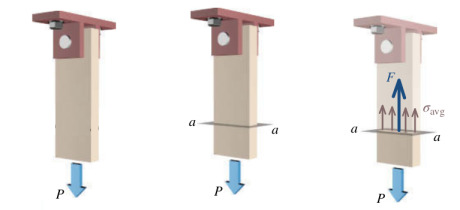
\includegraphics[width=8em]{phy_020_strs_01_01.jpg}

Nesne üzerindeki mavi noktalar bu seçilmiş noktaları gösteriyor.

Seçilmiş noktaların kordinatı bir referansa göre alınmalı, $e_1,e_2,e_3$
şeklinde bir baz bu işi yapabilir. Artık bu baza, kordinat sistemine izafi
olarak patates üzerindeki her noktayı bir vektör olarak temsil edebiliyoruz.
Altta örnek olarak üç tane seçiliş noktayı gösterdik,

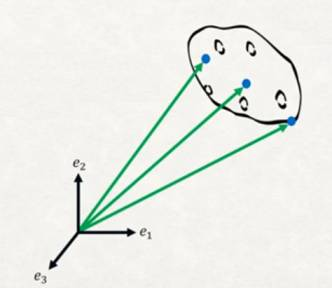
\includegraphics[width=13em]{phy_020_strs_01_02.jpg}

Daha fazla nokta da seçebilirdik, tüm seçilmiş noktalardan gelen vektörlerin
kümesi cisim hakkında bize bir konum, durum bilgisi verecektir, bu konuma biçim
değiştirme öncesi noktaların konumu $\Omega_0$ diyelim, ya da referans konumu.
Nesne üzerindeki değişimler, özellikle bu ders sonlu öğeler (finite elements
method, FEM) dersi olduğu için deformasyon değişimleri referans vektörlerinin
nasıl değiştiği üzerinden incelenebilir. İlk konumdaki bir vektörü, $X$ diyelim,
değişimi $f$ fonksiyonu yapıyor olsun, sonuç vektörü $x$ olacak, yani $x =
f(X)$.

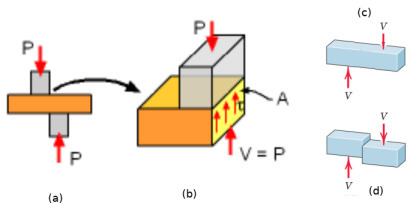
\includegraphics[width=17em]{phy_020_strs_01_03.jpg}

Üstteki resimde örnek bir değişim görüyoruz; yana kayma, dönme, uzama
var. Değişimi gerçekleştiren $f$ fonksiyonu. Bu ders için farz edilen $f$'nin
birebir ve örten (bijective) olduğu, liner cebirden hatırlarsak bu $f$'nin tersi
alınabilir olduğu anlamına geliyor, yani elimde deforme edilmiş konum var ise,
$f$'nin tersi ile başlangıç konumuna dönebilirim. Diğer bir faraziye fonksiyonun
sürekli (continuous), ve pürüzsüz (smooth), yani türevi alınabilir olduğu. Katı
cisim mekaniğinde türevi alınabilirlik önemli bir faraziyedir, gerçek hayatta
böyle mi, her zaman değil muhakkak, hatta bir bakıma bu sebepten dolayı FEM'e
ihtiyacımız var.

Ayrıca bize ileride lazım olabilecek bir üçüncü vektör $u$ da tanımlayabliriz,
bu vektör varılan konumu referans konumuna direk ilintilendiriyor. Vektör $u$'ya
yer değişim fonksiyonu denir. Pozisyon fonksiyonu ile karıştırmayalım, o küçük
$x$, bu yer değişim fonksiyonu $u$.

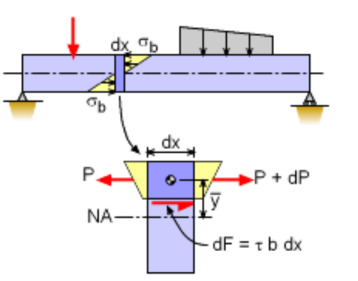
\includegraphics[width=17em]{phy_020_strs_01_05.jpg}

Fakat bu tüm grafiğe baktığımızda $u$'nun aslında vektör çıkartma operasyonunu
gösterdiğini fark edebiliriz, yani $u = x - X$.

Üç tür katı gövde değişimine bakalım şimdi, not katı demek gövde esneyip,
uzamıyor demek.

Katı Gövde Yer Değişimi: $x = X + c$, ki $c$ sabit bir vektör. Pür yer değişimi
olduğu için basit bir toplanma işlemi sadece. Şimdi bildiğimiz sonuç konumu
formülünü yazarsak, $u = x - X$ bu formülde önceki $x$'i geçirelim, $u = X + c -
X$ yani $u = c$.

Katı Gövde Dönüşü: $x = Q X$, formüldeki $Q$ bir dönüş matrisidir. Tekrar yer
değişim formülünü yazalım, $u = x - X$ ve önceki $x$'i yerine koyalım, $u = QX -
X$, tekrar düzenlersek, $u = (Q-I)X$.

Katı Gövde Hareketi: $x = QX + c$, bu kalem aslında önceki iki kalemin
birleşimi, hem dönüş hem de yer değişimi var. Çoğunlukla fizik problemlerinde bu
kavramdan bahsedilir. Yine $u$'yu düşünürsek $u = (Q-I)X + c$ elde ederiz.

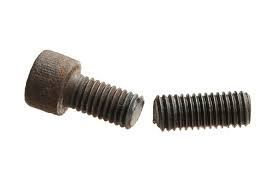
\includegraphics[width=10em]{phy_020_strs_01_04.jpg}

Üsttekiler değişim şekli ama hala gerinim, esneme, küçülme türü şekil
değişimlerini görmedik. Diğer değişimler şunlar,

Her Yönde Uzama ve Küçülme (Uniform Extension and Contraction)

Her kordinat ekseninde uzama var ise, mesela $x_1 = k_1 X_1$, $x_2 = k_2 X_2$,
$x_3 = k_3 X_3$, ki $k_i > 0$ reel sayı olmak üzere. Bu değişimleri matris
ile şöyle gösterebiliriz,

$$
x = \left[\begin{array}{c}
x_1 \\ x_2 \\ x_3
\end{array}\right] =
\left[\begin{array}{ccc}
k_1 & 0   &   0 \\
0   & k_2 & 0 \\
0   & 0   & k_3
\end{array}\right]
\left[\begin{array}{c}
X_1 \\ X_2 \\ X_3 
\end{array}\right] =
\left[\begin{array}{c}
k_1 X_1 \\ k_2 X_2 \\ k_3 X_3 
\end{array}\right]
$$

Ustteki ifadeden pozisyon fonksiyonunu soyle belirtebiliriz,

$$
u = x - X = \left[\begin{array}{ccc}
(k_1 - 1) X_1 \\ 
(k_2 - 1) X_2 \\ 
(k_3 - 1) X_3 
\end{array}\right]
$$

Eğer hem $k_1$ hem $k_2$ 1'den büyükse her iki eksende esneme görülürdü,

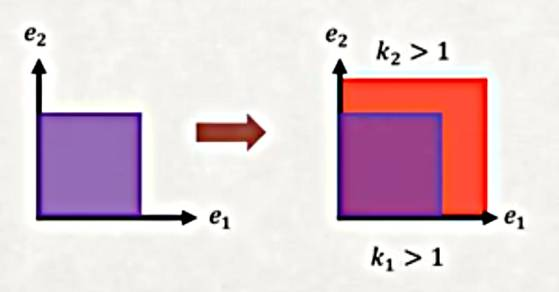
\includegraphics[width=10em]{phy_020_strs_01_06.jpg}

Eğer sadece $k_1 > 1$ ise o yönde büyüme olurdu, diğerinde değil. Eğer
$0 < k < 1$ ise küçülme, $k > 1$ ise büyüme, $k = 1$ değişim yok.

$k=0$ ya da $k<0$ fiziki dünyada mümkün değil, mesela $k<0$ durumunda nesnenin
tamamen kendi tersine dönmüş olması gerekiyor, bu da fiziksel olarak olamaz.

Basit Kaykılma (Simple Shear)

Üç boyutta $e_2$ etrafında bir kaykılma düşünüyor olsaydık, bunu

$$
x_1 = X_1 + k X_2, \qquad x_2 = X_2, \qquad x_3 = X_3
$$

ile temsil edebilirdik, $\theta$ açısında bir kaykılma için matris formunda

$$
x = \left[\begin{array}{ccc}
1 & \tan(\theta) & 0 \\
0 & 1 & 0 \\
0 & 0 & 1 
\end{array}\right]
\left[\begin{array}{c}
X_1 \\ X_2 \\ X_3
\end{array}\right] =
\left[\begin{array}{c}
X_1 + \tan(\theta) X_2 \\
X_2 \\
X_3
\end{array}\right] 
$$

$$
\implies u = x - X =
\left[\begin{array}{ccc}
\tan(\theta) X_2 \\
0 \\
0
\end{array}\right]
$$

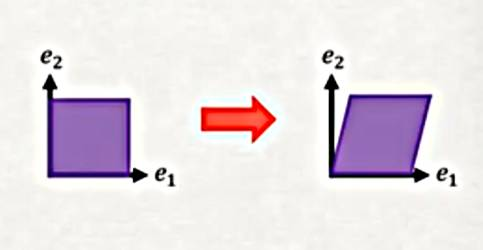
\includegraphics[width=10em]{phy_020_strs_01_07.jpg}

Pür Kaykılma (Pure Shear)

Bu tür şekil değiştirme birden fazla eksen bazında olabilir,

$$
x = \left[\begin{array}{ccc}
1               & \tan(\theta/2) & 0 \\
\tan(\theta/2) & 1              & 0 \\
0               & 0              & 1 
\end{array}\right]
\left[\begin{array}{c}
X_1 \\ X_2 \\ X_3
\end{array}\right] =
\left[\begin{array}{c}
X_1 + \tan(\theta/2) X_2 \\
\tan(\theta/2) X_1 + X_2  \\
X_3
\end{array}\right] 
$$

$$
\implies u = x - X =
\left[\begin{array}{ccc}
\tan(\theta / 2) X_2 \\
\tan(\theta / 2) X_1 \\
0
\end{array}\right]
$$

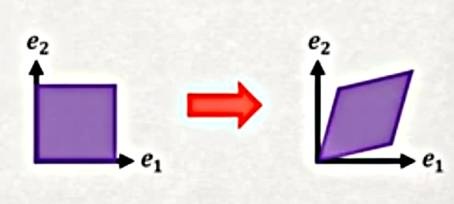
\includegraphics[width=10em]{phy_020_strs_01_08.jpg}

Nihayet gerilme konusunda geldik. Bu dersin en önemli konusu bu. Başta
gösterdiğimiz patatese dönelim, referans konumundaki bir mavi noktaya $X$'e
bakıyorduk, patatesi yamulttuğumuz zaman sonuç konumdaki $x$ elde ediliyordu,
her iki noktayı birbiriyle ilintilendiren aralarındaki $u$ vektörü idi.

Şimdi gerilme tensorunu türetmek için her patates için ikinci bir nokta
ekleyeceğiz. Referans konumda $X$ noktası ile bu ikinci nokta arasındaki vektör
$\ud X$ olacak, sonuç patatesindeki ikinci noktaya olan vektör $\ud x$.  Tabii
bu noktaları rasgele eklemedik, yamultan fonksiyon $\ud X$'i yamultunca için
$\ud x$ elde ettik, sonuç patatesteki ikinci noktaya böyle eriştik.

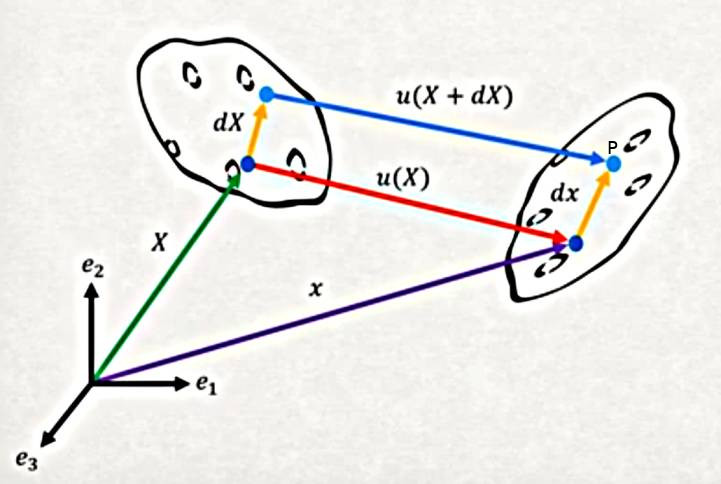
\includegraphics[width=15em]{phy_020_strs_01_09.jpg}

Şimdi diyelim ki orijinden ikinci patatesteki $P$ noktasına gitmek
istiyoruz. Bir yol $X$, $\ud X$, $u(X+\ud X)$ olabilirdi, bu vektörlerin toplamı
bizi $P$'ye götürür. Fakat daha kısa bir yol daha var, $x$, $\ud x$. Aynı
noktaya eriştiğimize göre bu iki yolun vektör toplamları birbirine eşit olmalı.
O zaman şu ifade doğrudur,

$$
x + \ud x = X + \ud X + u(X+\ud X)
$$







[devam edecek]

Kaynaklar

[1] Kim, {\em Introduction to Non-linear Finite Element Analysis}

\end{document}



